%
% Hypothesis - Dopamine \& Autism Spectrum Disorders
% 

% should reword

% DCN elided this section, due to an adequate summary of this material
% in the introduction section of the chapter.

% \subsection{Why Dopamine?} 
% The evidence for neurotransmitter abnormalities in ASD is varied, but, taken as a whole, worth further consideration.
% Abnormal DA levels have been demonstrated through many measures including PET, measures of DA metabolites such as homovanillic acid (HVA), and through the use of DA modulators in clinical trials demonstrating some mitigation of problematic behavior in ASD~\cite{FernellE:1997:AutismPET,MartineauJ:1992:AutismDopamine,TsaiLY:1999:AutismDopamine}.  Recently, studies have found potential genetic differences in specific dopamine receptors as well as evidence that differences in the morphology of the basal ganglia is potentially relevant in ASD~\cite{StaalW:2012:DopamineASDGenetics,QuiA:2010:ASDMotor}.  While the precise causal role, if any, that DA plays in autism is still an active area of investigation, this neurotransmitter does have interesting ties to numerous core deficits and related symptoms in autism spectrum disorders, including seizures~\cite{StarrMS:1996:SeizuresDA,TuchmanR:2002:EpilepsyAutism}, motor problems~\cite{RinehartNJ:2001:AutismMovement,RinehartNJ:2006:AutismGait}, repetitive behaviors~\cite{CanalesJJ:2000:Stereotypy,RalphRJ:2001:Perseveration,Ralph-WilliansRJ:2003:HyperactiveDA}, and neurogenesis~\cite{BortaA:2007:NeurogenesisDA}.  The ties of DA to autism are both numerous and compelling.  Further investigations into precisely how these differences affect behavior has great potential in providing a common language, that of neurobiology, for linking many disparate behaviors in people with ASD.

%Given the ample choices of brain areas to investigate, many with intriguing correlations to behavior in autism, why champion a closer look at the role of dopamine in opposition to any of the other implicated areas?  In truth there is, at this point, no ``smoking gun'' marking dopamine as a central cause of ASD.  However, dopamine does provide us with a unique opportunity to build a bridge between seemingly disparate and complex observed patterns of behavior in ASD.  Neurally, dopamine affects nearly all of the brain areas associated with autistic behavior, including the cerebellum, amygdala, PFC, parietal lobes, and the hippocampus~\cite{BarikS:1996:CerebellumDA,JacksonME:2001:AmygdalaDA,TessitoreA:2002:AmygdalaDA,MillerEK:2001:PFC,MehtaMA:2000:ParietalDA,LiS:2003:HippocampusDA}.  Behaviorally, numerous strong links exist between autism and dopamine.   

%\subsubsection{Evidence for Dopamine Dysfunction in ASD}
%The evidence for dopamine abnormalities in ASD is strong. Both PET imaging studies and urinalysis studies reveal differences in levels of dopamine in people with autism~\cite{FernellE:1997:AutismPET,MartineauJ:1992:AutismDopamine}.  However, clinical trials investigating the effects of both dopamine agonists and antagonists have had mixed results~\cite{PoseyDJ:2000:AutismDopamine,TsaiLY:1999:AutismDopamine}.  Many studies of drugs affecting brain levels of DA have shown improvements in stereotypic behaviors and other problem behaviors, but, some have shown an increase.  Studies involving clinical trials can be very difficult to evaluate.  For instance, at low doses, DA antagonists have been shown to actually have an agonistic effect on phasic dopamine release~\cite{FrankMJ:2006:Psychopharmacological}.  While it maybe difficult to interpret the clinical results, the data does strongly suggest a role for dopamine in the behavior of people with autism.  
%
%Coupled with these empirical results are many intriguing indirect correlates of DA dysfunction in autism as well.  These include 

%There are a number of different empirical results that support the idea that DA function plays an important role in autism.  These will be discussed next.  As isolated arguments, these results provide only weak support tying DA to ASD.  Taken together, however, they provide a strong case for seeing the DA system as key to understanding many of the behavioral patterns in autism. 

%A study of children born to mothers who used cocaine during their pregnancy provides indirect evidence for DA's role in the etiology of ASD.  11.4\% of children born to mothers who abused cocaine were diagnosed with autism, compared to an approximate 0.6\% prevalence rate in the general population.  Cocaine is known to affect the dopaminergic system, in particularly the substantia nigra as well as dopamine transporters, and can cause long term damage if used habitually~\cite{DavisE:1992:Cocaine}.  Recent studies have also linked cocaine use to an increased likelihood of acquiring Parkinson's disease~\cite{LloydSA:2006:Cocaine}.  The Parkinsonian study also shows a correlation which suggests that mothers who use cocaine during their pregnancy may put the child at higher risk for acquiring Parkinson's disease later in life.  This is interesting because Parkinson's disease is a disorder which results from degeneration of specific structures within the basal ganglia and the midbrain dopamine system, further strengthening the link between cocaine use by a pregnant woman and damage to dopaminergic system of her child.  However, in both the ASD and Parkinson's disease studies, we must be extremely careful not to make assumptions based on correlational data alone.  A much more rigorous analysis would be necessary before anything near to conclusive could be stated. 

%One of the most prescribed and investigated clinical drug treatments for autism are drugs which affect serotonin (5HT) levels. Benefits have been found similar to those shown in DA based drug trials, including reducing stereotypic behavior and improvements in other areas of disruptive behavior~\cite{PoseyDJ:2000:AutismDopamine,TsaiLY:1999:AutismDopamine}. At first glance, the benefits found by using various serotonin based treatments may be seen as an argument against any DA based deficit in autism.  Closer inspection shows this need not be the case. Many researchers have begun to investigate links between levels of 5HT and DA.  In particular, some theories view these two neurotransmitters as a coupled system, as opposed to each having a distinct and compartmentalized effect on behavior~\cite{DawND:2002:Opponent}. This coupling could explain why both DA and 5HT have been implicated in ASD. In particular, there is evidence concerning phasic 5HT encoding a prediction error in the same manner that the firing pattern of midbrain dopamine neurons have been found to encode a prediction error~\cite{DawND:2002:Opponent}.  The main difference, according to proponents of this account, is phasic 5HT encodes a prediction error in future \emph{punishments}, as opposed to future rewards, which DA is argued to encode. (See Section 2.3 for further explanation.).  The interactions between serotonin and dopamine systems are likely to be complex, but the payoffs for understanding the emergent properties of this possible coupling warrant further investigation. 

%\subsubsection{DA Ties to ASD Symptomology}
%	Dopamine has a role in many of the problematic behaviors demonstrated by people with autism.  These behaviors range from “lower-level”, non-intentional behaviors (such as seizures), to those at a much “higher-level”, such as learning to follow eye gaze and the ability to control and flexibly adapt our behavior.  The breadth of the links described below are, perhaps, the strongest argument for a closer examination of the causal role of dopamine in autism.

%Approximately 1 in 4 people with a diagnosis of autism will develop seizures during adolescence, significantly higher than the prevalence observed in the general population~\cite{TuchmanR:2002:EpilepsyAutism}.  In normally developing individuals, seizures occur approximately 1 in every 200 people. This indicates a more than ten-fold increase in ASD as compared to the general population.  For many decades, researchers have believed that dopamine plays a major role in epilepsy~\cite{StarrMS:1996:SeizuresDA}.  Anti-convulsant medications are known to have direct affects on the dopamine system, helping mitigate the seizures caused in epilepsy.  The link between DA and seizures further strengthens an argument for the possibility of a role of DA in ASD.

%People with autism also demonstrate a wide spectrum of motor abnormalities and problems. These problems range from problems initiating behaviors, repetitive movements, as well as abnormal gaits~\cite{RinehartNJ:2001:AutismMovement,RinehartNJ:2006:AutismGait,APA:2000:DSM4}. There are possibly large benefits to investigating the underlying  cause of the motor and movement abnormalities found in ASD, as well as understanding the possible social manifestations of these movement and motor difficulties. Not the least of these possible benefits could be a diagnostic criteria for autism containing specific observable behaviors to compliment the existing socially based standards~\cite{LearyMR:1996:Movement}. The basal ganglia and mesolimbic dopamine system are widely accepted as a vital component in learning and initiating motor movements. Problems within these brain areas are believed to be at the root of disorders, such as Parkinson's and Huntington's disease, which manifest problems in motor control, as well as other more cognitive symptoms.  Also, stimulation of the dopamine receptors located within the striatum has been shown to induce motor stereotypies, and ameliorated / abolished by blocking the dopamine transmission within the striatum~\cite{CanalesJJ:2000:Stereotypy,Ralph-WilliansRJ:2003:HyperactiveDA,RalphRJ:2001:Perseveration}. The link of motor control, movements, and motor problems to dopamine and dopamine producing areas is strong. Indeed, as mentioned, even stereotypic behavior, one of the triad of impairments currently needed for an autism diagnosis, has direct ties to dopamine. 

%\subsection{Neurogenesis}
%	Large brains, excessive growth.
%	Dopamine's role in neurogenesis, in particular brain growth.

%One of the earliest and most reliable predictors in autism-related language impairments and social performance is abnormalities in shared joint attention (SJA)~\cite{DawsonG:2004:SocialOrienting}. SJA can be defined as the ability to coordinate and follow attention between one's self, an object, and another person. The sharing of attention is often achieved by following eye gaze and pointing gestures in order to find a rewarding object in the environment. Problems with SJA are believed to be a key reason for the communicative and social deficits demonstrated by people with ASD. Recently, a formal account of how gaze following, and subsequently shared attention, is learned via interactions between an infant and caregiver has been proposed~\cite{TrieschJ:2006:GazeASD}. According to this account, SJA emerges naturally given only a very basic set of assumptions and mechanisms. At the core of these assumptions lies a learning account, inspired by reinforcement learning paradigms and precise neurobiological data. The reward based learning method employed by Triesch and colleagues, known as Temporal Difference or (TD) learning, has been strongly linked to the firing patterns of midbrain dopamine cells by other researchers~\cite{BartoAG:1994:TDLearning,MontaguePR:1996:Dopamine}. Leveraging this dopamine inspired learning method, Triesch et al. demonstrate how gaze following emerges naturally, with experience, given a simple structured environment and the aforementioned learning paradigm. Importantly, it is also shown how manipulating the reward structure reproduces problems in eye gaze following and shared attention as seen in people with ASD. The authors are careful to not make any unnecessary claims or assumptions as to the exact underlying biological  mechanism responsible for the theorized change.  However, as mentioned, the reward structure in models such as these is most often associated with the firing patterns of cells located within the midbrain dopamine system.  It is also worth noting that a recent extension of the model has been used to show how these same basic learning mechanisms can lead to cells, within a modeled supplementary motor area, with receptive field properties similar to ``mirror neurons''~\cite{TrieschJ:2007:Mirror}.  

%The ties of DA to autism are both numerous and compelling.  Further investigations into precisely how these differences affect behavior has great potential in providing a common language, that of neurobiology, for linking many disparate behaviors in people with ASD.

%\subsection{Dopamine \& Temporal Difference Learning}
%Our account of the role of dopamine in autistic behavior builds on past findings concerning the midbrain dopamine system and its relationship to the prefrontal cortex. Analyzing the response profile of DA neurons in the basal ganglia of monkeys, Schultz et al. (1997)~\nocite{SchultzW:1997:TD} demonstrated DA cells can encode a prediction error in the amount of future reward expected to be given to the monkey.  In other words, these cells seem to encode a \emph{change in expected future reward}.  Figure~\ref{schultz} shows results from a population of midbrain DA cells during one of Schultz's experiments.  The top panel represents the situation in which the monkey is not expecting reward, but then receives reward (e.g., a sip of juice).  Notice that the DA cells fire upon receiving the reward (signified by ``R'' on the graph), encoding a positive change in what the monkey was expecting.  In the bottom left panel, the monkey has now been conditioned to associate a flash of light with the delivery of the juice, after a short delay.  In other words, the monkey now knows that the flash of light predicts future reward.  When the flash of light is seen (represented as ``CS'', for ``conditioned stimulus'', in the graph), the DA cells fire.  This can be explained as the monkey expecting future reward once the light comes on, signaling that juice is expected to be coming soon: a positive change in expected future reward.  However, when the reward is delivered (``R'') the cells to do not fire, since the monkey was already expecting reward.  When the juice is delivered there is no change in expected future reward, in this case, and, therefore, no increase in the rate of DA firing.  In the panel located at the bottom right, the DA cells again fire for the flash of light (``CS'', conditioned stimulus) , but this time the experimenters \emph{withhold the juice} at the time when the monkey is expecting the juice to be delivered.  The monkey is \emph{expecting} reward, but no reward is delivered. Thus, at the time that juice is expected, there is a negative going change in expected future reward.  Notice that the firing rates of the DA cells around the expected delivery time of reward (``R'') actually dip below their baseline firing rate and, indeed, appear to encode this negative change in expected future reward.

%This is very interesting because change in expected future reward is also the key variable in a very powerful reinforcement learning algorithm known as Temporal Difference (TD) learning.  In TD learning, the change in expected future reward, the same value the DA cells appear to be encoding, is know as the TD Error.  Across two consecutive time steps the TD Error is given by: 
%\begin{equation}\delta(t) = r(t) + \gamma V(t+1) - V(t)\end{equation}

%Where $r(t)$ is a continuous reward value that is delivered at each time step based on system performance (e.g., $r(t) = 1$ for correct performance and $r(t)=0$ on time steps when no reward is presented), $V(t)$ and $V(t+1)$ are the expected future rewards at times $t$ and $t+1$ respectively, \begin{math}\delta(t)\end{math} is the change in expected future reward, or TD Error, and \begin{math}\gamma\end{math} is a constant discounting factor, where \begin{math}0 < \gamma \leq 1\end{math}.  Adjusting \begin{math}\gamma\end{math} changes the amount by which temporally distant rewards are discounted as compared to rewards that can be attained in the temporally near future. 

%This connection has led researchers to formalize the role of midbrain DA neurons in the brain's learning mechanisms~\cite{BartoAG:1994:TDLearning,MontaguePR:1996:Dopamine}, equating the firing rate of the DA cells with the amount of change in expected future reward, or TD Error.  Neurally plausible implementations of TD learning have been implemented and have been used to model the learning of motor sequences in the striatum~\cite{MontaguePR:1996:Dopamine}, driven by the reward-prediction DA signal.


%\begin{figure}
% 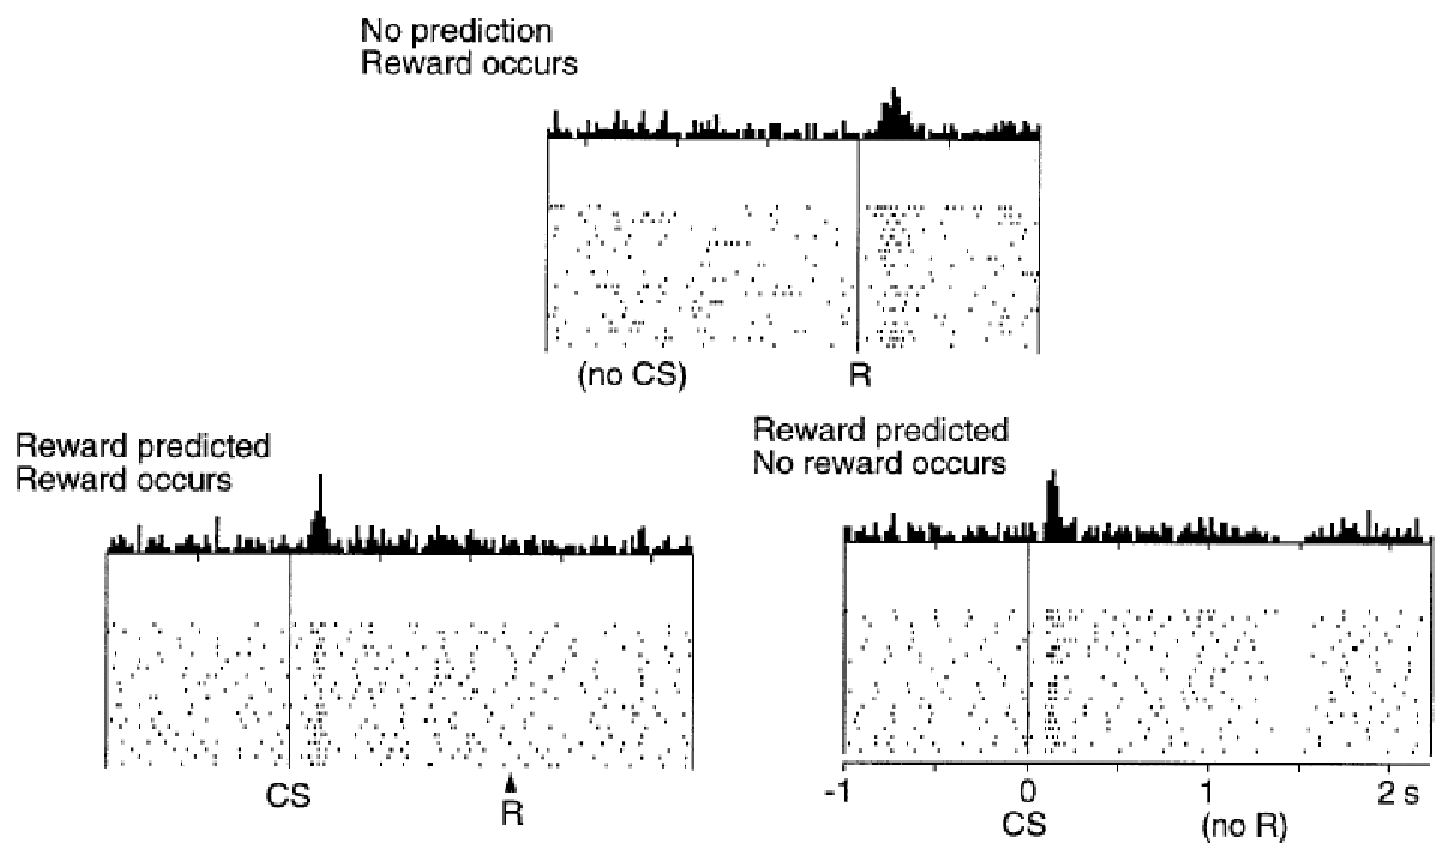
\includegraphics[width=15cm]{figures/schultz}
% \caption{Firing rates of midbrain dopamine neurons of the basal ganglia during classical conditioning (Adapted from Schultz et al., 1997)}
% \label{schultz}
%\end{figure}


%\bigskip

%\subsection{Computational Models of PFC}
%Our work builds on previous computational modeling work of formal accounts of DA's affect on PFC functioning.  The effect of DA is formalized by equating the firing rate of midbrain DA neurons to the key variable, the TD Error, of the powerful TD learning algorithm.  Using this connection between biology and machine learning, researchers have been able to provide models of how motor systems can learn sequences of overt actions leading to reward.  One of the primary insights of some recent models of PFC functioning is that the DA based TD learning mechanism might be used to learn, from experience, when to robustly maintain current representations in the PFC versus allowing updating to occur~\cite{BraverTS:2000:Control}.  As described earlier, it is helpful to think of the maintenance versus updating of PFC in terms of a gating mechanism.  When the gate is closed, the PFC representations are robustly maintained and protected from interference.  When the task contingencies change, the gate can be opened to allow for a more useful PFC goal or rule to be maintained to influence further processing.  The key insight is that, if TD can be used to learn sequences of \emph{overt} actions, it might be possible to use this same error signal to learn \emph{covert} actions, such as when to open and when to shut the gate on PFC representations.  By building computational models of PFC function, researchers have shown that this account is plausible~\cite{BraverTS:2000:Control,OReillyRC:2002:IDED}.  A layer of processing units representing  the PFC is included in these models, and this layer is used to actively maintain abstract task dimensions across the firing patterns of the units.  For instance, the PFC layer can encode, and actively maintain, a representation such as ``pay attention to the color of the stimuli''.  This maintained pattern of activity can then provide a ``top-down'' bias or up-modulation of pathways in posterior brain areas associated with the processing of stimulus color~\cite{CohenJD:1990:Stroop}.  The extra biasing provided by the PFC can be used to drive weaker, less automatic, behaviors (e.g. naming the color as opposed to reading the word in the Stroop task) when appropriate.  This activation based modulation is thought to be key to our ability to provide cognitive control over behavior~\cite{CohenJD:1992:Schizophrenia}.  The DA based adaptive gating mechanism can be used, within this context, as a way to signal to PFC when it is appropriate to strengthen the maintenance of the representation currently encoded (i.e. close the gate).  This occurs when a positive TD Error arises, signifying a positive change in expected future reward.  In other words, when the system is doing better than expected, close the gate on PFC representations so we are more likely to keep doing the same thing.  Conversely, when the network starts performing worse than expected, possibly due to task contingencies changing, this will result in a negative TD Error, signaling that the system is not performing as well as expected, and indicating that the system should adapt its behavior to perform more optimally.  The negative TD error can be used as a gating signal on the PFC representations, signaling the gate to open, allowing a new representation to replace the old, thereby allowing the network to flexibly adjust its control over behavior.
%
%Along with providing a neural mechanism that can learn to appropriately and adaptively gate PFC representations, these models have also been successful in tying frontal disturbances, such as those found in schizophrenia, to deficits in cognitive control~\cite{CohenJD:1992:Schizophrenia} and cognitive flexibility~\cite{BraverTS:1999:Schizophrenia,OReillyRC:2002:IDED}.  A recent elaboration of this model, XT~\cite{RougierNP:2005:XT}, is the first neuroscientific model able to provide quantitative fits to a hallmark task of cognitive control, the Stroop task, and a widely used measure of cognitive flexibility, WCST, in both neurologically intact and frontally damaged people.  
%In the next chapter, XT has been adapted to investigate whether a dysfunctional DA based gating mechansim can capture the specific executive profile of people with autism in WCST and Stroop.  

